\documentclass[11pt,a4paper]{article}

% --- Packages ---
\usepackage[utf8]{inputenc}
\usepackage[T1]{fontenc}
\usepackage{mathptmx}
\usepackage[margin=1in]{geometry}
\usepackage{amsmath, amssymb, amsthm}
\usepackage{graphicx}
\usepackage{booktabs}
\usepackage{hyperref}
\usepackage{xcolor}
\usepackage{authblk}

% --- Hyperref settings ---
\hypersetup{
  colorlinks=true,
  linkcolor=black,
  citecolor=black,
  urlcolor=blue,
  pdftitle={Information Field Geometry Theory},
  pdfauthor={Yuhki Endoh}
}

% --- Title and author ---
\title{\textbf{Information Field Geometry Theory}\\[0.3em]
\large\itshape The Geometry of Quasi-Closure}

\author{Yuhki Endoh}
\affil{Independent Researcher}

\date{April 30, 2026}

\begin{document}

\maketitle

\begin{abstract}
This paper proposes Information Field Geometry Theory (IFGT). IFGT is a framework for describing information not as a substance or a description of states, but as a \emph{quasi-closure}: a residual structure that persists when difference does not fully close in the process of approaching closure.

The theory builds on Vortical Enclosure Dynamics (VED), which describes the generation of physical structure from difference, gradient, flow, and closure. Within the same generative process described by VED, IFGT treats the persisting unclosed structure as information. While VED describes physical persistence realized through the closure degree $C$, IFGT addresses the complementary side---what fails to fully close---as information. In this framing, information is not opposed to physical structure but is a complementary aspect of the same generative structure.

IFGT introduces five basic variables: information density $I$, information flow $J$, information potential $\Phi$, informational time $\tau$, and the generation term $\sigma$. The relation between $I$ and $C$ is given by $I = f(1 - C)$, and $\sigma$ is defined as the mismatch between the current difference chain and the existing trace structure. In the final chapter, these components are integrated into a unified VED$\times$IFGT equation, yielding a single evolution equation for the closure-degree field $C(x,\tau)$.

Within this framework, information is not a static object of description but a dynamic process that participates in structural formation through the persistence of difference and the constraint of flow. IFGT thus provides a foundational theory for describing the general structure that may encompass informational behavior observed in biological and computational systems.
\end{abstract}


\section{Introduction}
\label{sec:introduction}

The Information Field Geometry Theory (IFGT) proposed in this paper is a framework for describing information not as a substance but as a geometric structure. IFGT is not an independent foundational theory; it is positioned as an upper-layer effective theory built upon Vortical Enclosure Dynamics (VED), which describes the generation of physical structure from difference, gradient, flow, and closure.

Information has traditionally been understood primarily as a description of states. When modern physics claims that ``matter is also information,'' this information typically functions as a label attached to the state of a system. The information treated in this paper differs from this usage. Here, information refers to a \emph{structural constraint} arising as a trace left behind when difference does not fully dissipate. Such information has no independent substance; it acts by constraining the paths and distributions of difference chains.

Information is not difference itself. Information appears when difference persists in a distinguishable form and becomes referable in relation to other differences. In this sense, information is a trace produced by the persistence of difference and functions as a scaffold for subsequent difference chains. Information is, therefore, the structure that makes the chaining of differences possible.

This structure is not fully closed; rather, it appears as a fluctuation of difference that cannot be eliminated in the process of approaching closure. In this theory, we call such a structure a \emph{quasi-closure}. A quasi-closure retains differences, produces gradients, and induces flows, thereby forming structure. At the same time, this structure is not separated from physical persistence but interacts with it within the same generative process.

This interaction is not unidirectional but circular. The informational structure as a quasi-closure constrains difference chains, biases their flow, and thereby participates in the formation of new structure. The resulting structure manifests as physical persistence and generates further differences. When these differences in turn remain as quasi-closures, information and matter are generated cyclically, transforming into one another.

Information does not exist statically; it becomes manifest at boundaries where structural change occurs. Such a boundary functions as a front of change and affects the direction and intensity of difference chains. This boundary structure is especially prominent in biological and computational systems, where the interference of past traces with present change is observed as fluctuations of behavior or state.

Such information is concretely implemented in the nervous systems of organisms, the memory of computers, and the internal states of transformer models. These are not information itself but instances in which the structure that retains traces of difference and constrains flow is realized within a physical system. This paper does not address these specific implementations but aims to describe the general structure underlying them.

Thus, the information in this theory is understood as a structure of difference that persists in the process of approaching closure. This structure is described as a geometry that produces the flow and constraint of differences. IFGT provides a framework to describe this informational geometric structure with a minimal set of variables and relations.

\subsection{On the notion of information}
\label{subsec:notion_of_information}

The term \emph{information} is used with considerably different meanings across disciplines, and the position of this paper should be located within that landscape. We here organize four principal notions.

\paragraph{Shannon information.}
In information theory, information is defined as a reduction of probabilistic uncertainty, quantified by $H = -\sum_i p_i \log p_i$. Meaning and weight are intentionally excluded from the formalism. This makes the theory mathematically powerful and domain-independent, but it does not address what information \emph{is}, only how much of it is transmitted.

\paragraph{Physical information (``It from Bit'').}
In the tradition of Wheeler and Landauer, information is treated as a label attached to the state of a physical system, with measurable consequences such as thermodynamic cost of erasure. This formulation is rigorous, but its scope is constrained by the requirement of observability: only quantities that can be measured as physical observables enter the theory. As a consequence, aspects of information such as weight (the degree to which a particular informational structure shapes subsequent dynamics) and semantic interactions below a certain threshold tend to be excluded, not because they are absent, but because they are not directly captured by the available measurement formalism.

\paragraph{Affordance (Gibson).}
In ecological psychology, Gibson~\cite{gibson1986} proposed that information resides not in the environment alone nor in the perceiver alone, but in the relational structure between them. An affordance---the possibility of action offered to an organism by its environment---carries a weight that is determined dynamically by context, rather than as a fixed physical magnitude. This captures an aspect of information that the physical formulation cannot: relationality, context-dependence, and dynamic weighting. However, the notion has remained largely descriptive and has not been given a dynamical formulation.

\paragraph{The informal notion.}
In everyday usage, information is something that persists as meaning and continues to influence subsequent states. This notion is closer to the structural and dynamic aspects that the strict physical formulation leaves out, and it retains the relational character emphasized by affordance.

\paragraph{Position of this paper.}
The information treated in IFGT is not Shannon information, nor a physical state label, but can be understood as a dynamical formulation of the relational structure suggested by affordance and by the informal notion. Concretely, it refers to the \emph{structural constraint that persists as a quasi-closure}---a residue of difference that has not fully closed and that biases subsequent difference chains. The weight of such information is expressed geometrically, as the local depth of the closure-degree field $C$ (see~§\ref{subsec:asymmetry} and~§\ref{subsec:circulatory_structure}). In this sense, IFGT aims to provide a dynamical description of the informational structure whose relational and weighted character has been recognized, but not formalized, in the preceding traditions.


\section{Relation to VED}
\label{sec:ved_relation}

\subsection{Division of roles}
\label{subsec:division_of_roles}

IFGT is not an independent foundational theory but an upper-layer effective theory that describes the \emph{unclosed side} of the generative structure described by Vortical Enclosure Dynamics (VED).

The division of roles between VED and IFGT is organized as follows.

\begin{itemize}
  \item \textbf{VED}: Describes the \emph{generation} of physical structure from difference, gradient, flow, and closure. It treats stable structures, particles, fields, and spacetime that are realized through the closure degree $C$.
  \item \textbf{IFGT}: Within the same generative structure, treats the informational structure that persists as a \emph{quasi-closure} in the region where $C$ does not reach unity.
\end{itemize}

VED addresses the side where closure succeeds; IFGT addresses the side where closure remains incomplete. The two are not opposing theories but complementary descriptions of the same generative structure viewed from different aspects. This division is visualized in Fig.~\ref{fig:two_aspects}.

\begin{figure}[h]
  \centering
  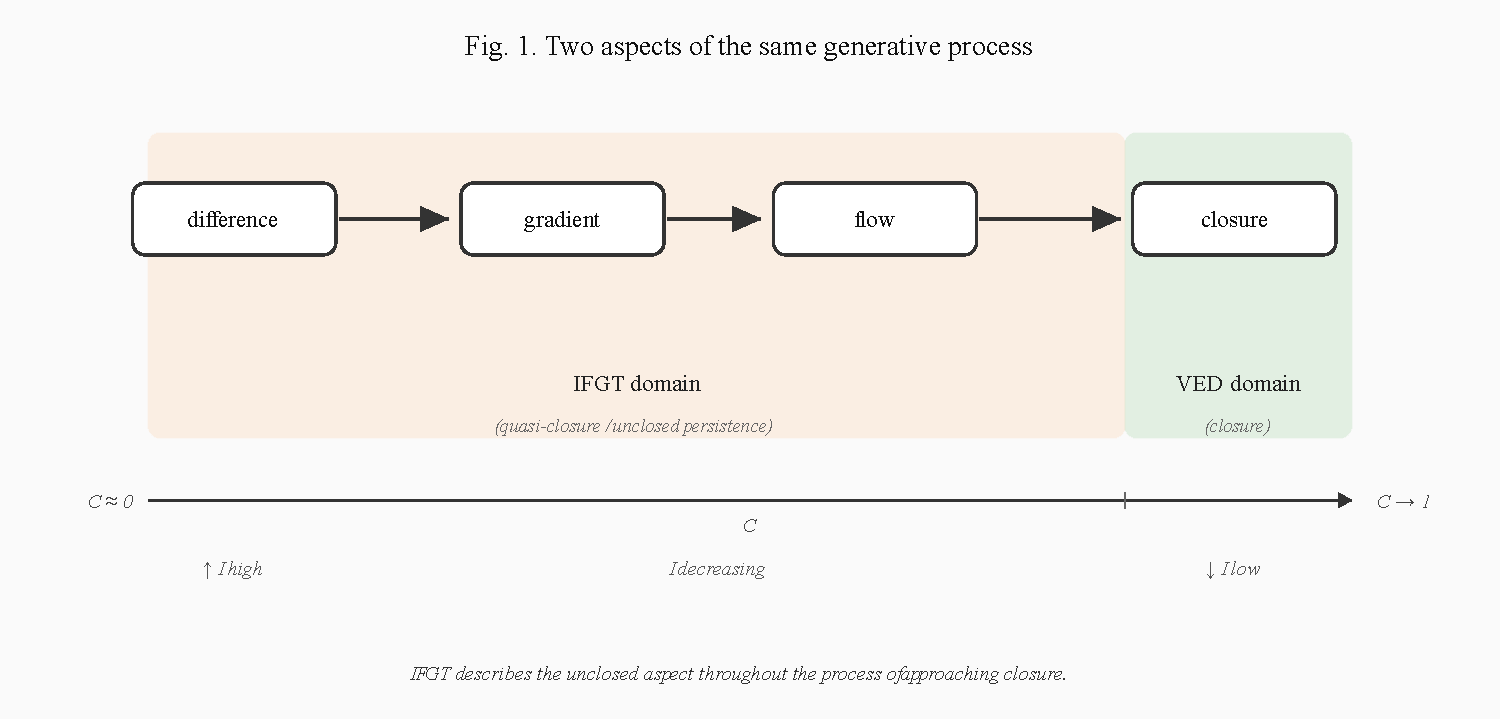
\includegraphics[width=0.95\textwidth]{figures/fig1_two_aspects_en.pdf}
  \caption{Two aspects of the same generative process. The VED chain (difference $\to$ gradient $\to$ flow $\to$ closure) unfolds across the closure-degree axis $C$. IFGT covers the region where $C$ has not yet reached unity; VED describes the fully closed region.}
  \label{fig:two_aspects}
\end{figure}

\subsection{The asymmetry between \texorpdfstring{$I$}{I} and \texorpdfstring{$C$}{C}}
\label{subsec:asymmetry}

The central quantity of VED is the closure degree $C \in [0, 1]$. The central quantity of IFGT, the information density $I$, is related to $C$ by
\begin{equation}
I = f(1 - C),
\label{eq:I-C-relation}
\end{equation}
where $f$ is a non-decreasing function satisfying $I \to 0$ as $C \to 1$. In the region of complete closure, where $C$ reaches unity, information does not exist; information is defined only in the region where $C < 1$.

This relation shows that $I$ and $C$ are \emph{not two expressions of the same quantity but complementary quantities}. $C$ describes ``the degree of closedness,'' while $I$ describes ``the density of the residue that failed to close.'' Both arise from the same field but can behave as independent quantities (for example, two regions with the same $C$ may have different spatial distributions of $I$ depending on their history).

This asymmetry is precisely what embodies the division of roles between VED and IFGT at the level of variables.

\subsection{Informational time \texorpdfstring{$\tau$}{tau} and generative time \texorpdfstring{$\tau_{\mathrm{VED}}$}{tau-VED}}
\label{subsec:time}

Three notions of time appear in this paper; we organize them here.

\begin{itemize}
  \item \textbf{Ordering parameter $t$}: an externally given time axis. It is meaningful only in the effective description where the background spacetime is fixed (see~§\ref{sec:unified_equation}).
  \item \textbf{Generative time $\tau_{\mathrm{VED}}$}: the observational time of VED Vol.~1. It is defined endogenously as the progression of difference consumption accompanying closure formation.
  \item \textbf{Informational time $\tau$}: the time introduced in IFGT. It is defined endogenously as the accumulation of \emph{mutual interference between difference and the existing trace structure}.
\end{itemize}

$\tau_{\mathrm{VED}}$ and $\tau$ \emph{differ in origin}. The former advances as closure proceeds; the latter advances as traces are updated.

Nevertheless, the two are \emph{dynamically isomorphic}. Both are not externally given parameters but quantities generated endogenously from the internal difference dynamics of the system, and both are irreversible. Accordingly, this theory treats IFGT's $\tau$ as a quantity embeddable on the same temporal axis as VED's $\tau_{\mathrm{VED}}$. It should be noted, however, that the two quantities measure different aspects of the same phenomenon and cannot be fully identified.

\subsection{The circular relation}
\label{subsec:circular}

The relation between VED and IFGT is not a unidirectional reduction. The informational quasi-closure is not merely added on top of physical structure; through its mutual interference with physical structure, it alters subsequent difference generation and flow. Conversely, physical structure produces new differences, which in turn form informational structures as quasi-closures.

\begin{equation}
\text{difference}
\xrightarrow{\text{partial closure}}
\text{quasi-closure (IFGT)}
\xrightarrow{\text{constraint}}
\text{structure (VED)}
\xrightarrow{\text{regeneration}}
\text{difference}
\label{eq:cycle}
\end{equation}

This cyclic relation is depicted in Fig.~\ref{fig:cyclic_relation}.

\begin{figure}[h]
  \centering
  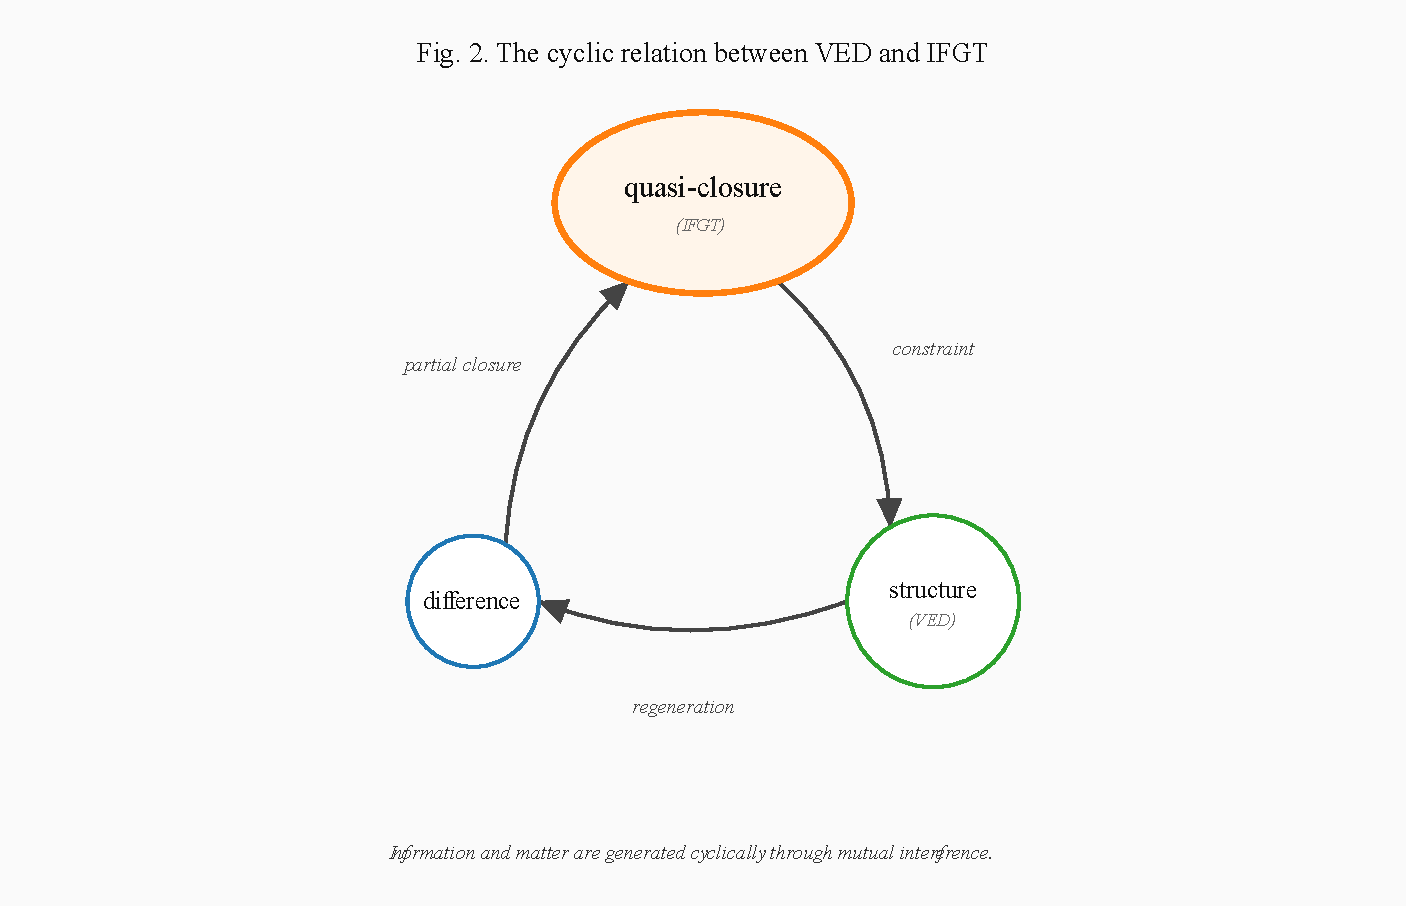
\includegraphics[width=0.80\textwidth]{figures/fig2_cyclic_relation_en.pdf}
  \caption{The cyclic relation between VED and IFGT. Information and matter are generated cyclically through mutual interference. The quasi-closure is positioned as the central mediating node.}
  \label{fig:cyclic_relation}
\end{figure}

This cycle is particularly prominent in the nervous systems of organisms, the memory of computers, and the internal states of transformer models, all of which are concrete examples of quasi-closures in which traces of difference are retained and subsequent flows are biased. This paper does not address these specific implementations but aims to describe the general structure underlying them.


\section{Correspondence with VED}
\label{sec:correspondence}

The division of roles described in the previous section is now organized in terms of variable correspondence and dynamical correspondence.

\subsection{Variable correspondence table}
\label{subsec:variable_table}

\begin{table}[h]
  \centering
  \begin{tabular}{l l l}
    \hline
    \textbf{VED} & \textbf{IFGT} & \textbf{Relation} \\
    \hline
    closure degree $C \in [0,1]$ & information density $I$ & $I = f(1 - C)$ \\
    difference $\Delta$ & information difference $\delta I$ & difference residue as trace \\
    gradient $\nabla C$ & information gradient $\nabla I$ & opposite direction via $I = f(1-C)$ \\
    closure flow $J_C$ & information flow $J$ & different aspects of the same flow \\
    closure potential & information potential $\Phi$ & $\Phi = -\alpha C + \Phi_0$ \\
    generative time $\tau_{\mathrm{VED}}$ & informational time $\tau$ & different origin, dynamically isomorphic \\
    --- & generation term $\sigma$ & corresponds to VED's difference generation \\
    \hline
  \end{tabular}
  \caption{Variable correspondence between VED and IFGT.}
  \label{tab:variable_correspondence}
\end{table}

\subsection{Difference \texorpdfstring{$\Delta$}{Delta} and information difference \texorpdfstring{$\delta I$}{delta I}}
\label{subsec:difference}

In VED, the difference $\Delta$ is a primitive quantity derived directly from the foundational axiom ``\emph{there is difference}'' and serves as the driver of closure formation. In IFGT, the information difference $\delta I$ is the residual difference that remains when difference does not fully close.

Whereas $\Delta$ is unprocessed difference itself, $\delta I$ is interpreted as ``the part that did not contribute to closure.'' The following relation therefore holds:
\begin{equation}
\Delta = \Delta_{\to C} + \delta I,
\label{eq:delta_decomposition}
\end{equation}
where $\Delta_{\to C}$ is the component of difference that contributes to closure and $\delta I$ is the component that persists as a quasi-closure.

\subsection{Structural correspondence}
\label{subsec:structural_correspondence}

In VED, difference produces gradient, gradient produces flow, and flow forms closure, giving rise to structure as physical persistence.

In IFGT, when difference does not fully close, it persists as a quasi-closure. This quasi-closure accumulates as a trace, constituting the information density $I$. The non-uniformity of traces produces the information gradient $\nabla I$, which drives the information flow $J$. Furthermore, the accumulation of quasi-closures constrains the flow, which is described as the information potential $\Phi$.

\subsection{Dynamical correspondence}
\label{subsec:dynamical_correspondence}

\begin{table}[h]
  \centering
  \begin{tabular}{l l l}
    \hline
    \textbf{Aspect} & \textbf{VED} & \textbf{IFGT} \\
    \hline
    structure & closure (stable, tending to rest) & quasi-closure (circulatory, persisting motion) \\
    terminal state & complete closure $C \to 1$ & metastable circulation \\
    time evolution & closure formation & trace update \\
    \hline
  \end{tabular}
  \caption{Dynamical correspondence between VED and IFGT.}
  \label{tab:dynamical_correspondence}
\end{table}

Closure is a stable structure tending toward rest, whereas a quasi-closure forms a circulatory structure while maintaining flow. This circulation strengthens local constraints and draws in surrounding flow.

\subsection{Generation and mismatch}
\label{subsec:generation_mismatch}

The generation term $\sigma$ in IFGT represents the mismatch between the current difference chain and the existing quasi-closure structure. This mismatch corresponds to the generation of new differences in VED and induces the update of structure.

Thus the generation of difference in VED and the generation through $\sigma$ in IFGT are different descriptions of the same process.


\section{Fundamental Dynamics}
\label{sec:fundamental_dynamics}

IFGT is a theory that describes motion within a quasi-closure, which appears as a fluctuation of difference that does not fully close. A quasi-closure is not separated from physical structure but interacts with it within the same generative process. Through this mutual interference, the informational quantities evolve in time.

This section defines the basic variables of the information field and introduces their evolution equations.

\subsection{Definition of basic variables}
\label{subsec:basic_variables}

\paragraph{Information density $I$.}
The information density $I$ is the density of traces left behind when differences fail to dissipate---the accumulation of persisting history. As stated in the previous section, $I$ is related to VED's closure degree $C$ by $I = f(1 - C)$.

\paragraph{Information flow $J$.}
The information flow $J$ is a vector quantity representing the direction and manner in which difference propagates. It describes the paths and distributions of change within a quasi-closure.

\paragraph{Information potential $\Phi$.}
The information potential $\Phi$ is a scalar quantity representing the strength with which the information flow is constrained and biased toward specific paths. It acts as interference with fluctuations and restricts the degrees of freedom of difference chains. The relation between $\Phi$ and $C$ is given by $\Phi = -\alpha C + \Phi_0$, where $\alpha$ is the constraint coupling constant and $\Phi_0$ is an arbitrary constant (which vanishes under the gradient and thus does not contribute to the dynamics).

\paragraph{Informational time $\tau$.}
The informational time $\tau$ is defined as the progression accumulating through the mutual interference between difference and physical structure. It is not an externally given parameter but is generated endogenously from the interaction between difference chains and structural constraints (see~§\ref{subsec:time}).

\paragraph{Generation term $\sigma$.}
The generation term $\sigma$ is the quantity representing the mismatch between the current difference chain and the existing informational trace structure. Such mismatch arises when the compatibility between structure and flow breaks down, inducing the generation of new differences and changes in the information density. The concrete construction of $\sigma$ is developed in Section~\ref{sec:unified_equation}.

\subsection{Basic equation}
\label{subsec:basic_equation}

The time evolution of the information density is determined by transport via the information flow and by the generation term:
\begin{equation}
\frac{\partial I}{\partial \tau} + \nabla \cdot J = \sigma.
\label{eq:basic}
\end{equation}

The first term on the left represents the time change of information density, and the second term represents the transport effect due to the divergence of the information flow. The right-hand side $\sigma$ represents the difference generation due to mismatch.

\subsection{Construction of the information flow}
\label{subsec:info_flow}

The information flow is specified by the gradient of trace density and by the information potential:
\begin{align}
J &= -D \nabla I + \mu F_I, \label{eq:J}\\
F_I &= -\nabla \Phi = \alpha \nabla C. \label{eq:F_I}
\end{align}

Here $D$ is the diffusion coefficient, $\mu$ the potential response coefficient, and $\alpha$ the constraint coupling constant. The first term represents a diffusive flow that resolves the non-uniformity of trace density; the second term represents a flow following the potential gradient.

The $F_I$ given by \eqref{eq:F_I} acts as a \emph{constraint force} drawing the information flow toward specific paths through the gradient of the closure degree. In regions where $\nabla C$ is large (the boundaries of closure), strong constraint is exerted and the flow is drawn in.

\paragraph{Terminology.}
The structure expressed by \eqref{eq:F_I}---``the gradient of the closure degree draws in the flow''---could, by analogy with existing physics, be called \emph{information gravity}. This is a useful designation that aids intuitive understanding: if $\nabla C$ is read as $\nabla \Phi_{\mathrm{grav}}$, then it plays formally the same role as the potential gradient in Newtonian gravity.

However, this paper does not identify $F_I$ with gravity in the usual sense (a force arising from the curvature of spacetime). We treat it solely as a potential gradient that geometrically constrains the degrees of freedom of difference chains. In what follows, we therefore prioritize descriptive clarity and unify the terminology as ``\emph{constraint potential gradient}'' or ``\emph{information-geometric force}.'' The designation \emph{information gravity} may be used for intuitive explanation or as a bridge to other domains, but within the internal description of the theory we adopt the vocabulary of information geometry.

\subsection{Quasi-closure and circulatory structure}
\label{subsec:circulatory_structure}

When the bias of informational traces grows stronger, the fluctuations of the difference chain become fixed along specific paths, and the degrees of freedom of flow decrease. However, since complete closure is not attained, the flow does not stop; instead, it forms a circulatory structure.

This circulation strengthens local constraints and draws in surrounding flow. As a consequence, this structure can be described as possessing \emph{inertial properties}. The mass-like quantity in IFGT is characterized by the local depth of $C$ (closure strength) and is understood as the degree of update resistance.


\section{The Unified VED$\times$IFGT Equation}
\label{sec:unified_equation}

The evolution equation~\eqref{eq:basic} of the information field introduced in the previous section does not specify the concrete construction of $\sigma$. In this section, we expand $\sigma$ as the mismatch between the difference chain and the existing trace structure, and ultimately unify the formulation into a single equation for VED's closure-degree field $C(x,\tau)$.

\subsection{Expansion of the generation term \texorpdfstring{$\sigma$}{sigma}}
\label{subsec:sigma_expansion}

$\sigma$ consists of three contributions.

\paragraph{(i) Driving term --- supply of unclosed difference.}
In regions where differences have not yet been incorporated into closure, new quasi-closures are generated. This contribution is proportional to the closure margin $(1 - C/C_*)$ and the difference source $\Delta$:
\begin{equation}
\sigma_{\mathrm{drive}} = a \, \Delta \, \left(1 - C/C_*\right).
\label{eq:sigma_drive}
\end{equation}
Here $\Delta$ denotes the difference source in VED (see~§\ref{subsec:difference}), $a$ is the generation rate, and $C_*$ is the effective closure upper bound. As $C \to C_*$, the driving vanishes.

\paragraph{(ii) Dissipation term --- collapse of traces.}
Quasi-closures decay over time, either being reabsorbed into closure or being released again as difference. This contribution is proportional to the trace density (equivalently, the local strength of $C$):
\begin{equation}
\sigma_{\mathrm{dissip}} = -\Gamma \, C,
\label{eq:sigma_dissip}
\end{equation}
where $\Gamma$ is the dissipation rate.

\paragraph{(iii) Barrier term --- the prohibition of complete closure.}
As a basic principle of VED, complete closure at $C = C_{\max} = 1$ is prohibited. This is a structural constraint that follows from the foundational axiom ``\emph{there is difference}.'' The prohibition is expressed as a repulsive potential that diverges as $C \to C_{\max}$:
\begin{equation}
\sigma_{\mathrm{barrier}} = -\frac{\kappa_B}{C_{\max} - C},
\label{eq:sigma_barrier}
\end{equation}
where $\kappa_B$ is the barrier strength. This term prevents asymptotic approach to complete closure and ensures circulation as a quasi-closure.

The three contributions are visualized in Fig.~\ref{fig:sigma_decomposition}.

\begin{figure}[h]
  \centering
  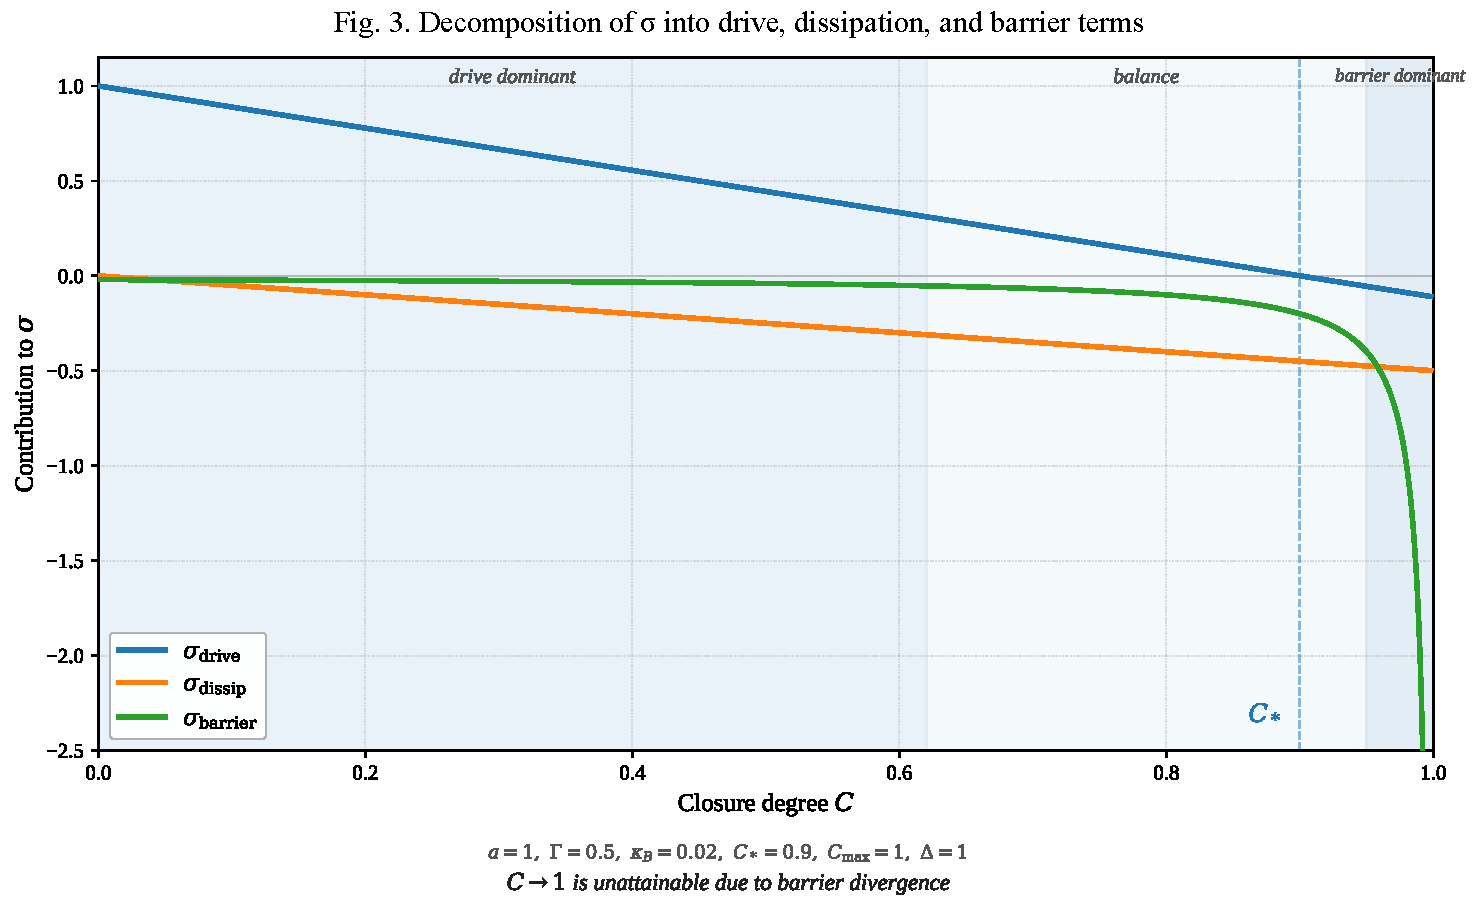
\includegraphics[width=0.95\textwidth]{figures/fig3_sigma_decomposition_en.pdf}
  \caption{Decomposition of $\sigma$ into drive, dissipation, and barrier terms. The barrier term diverges as $C \to 1$, ensuring that complete closure is unattainable.}
  \label{fig:sigma_decomposition}
\end{figure}

\subsection{The unified VED$\times$IFGT equation}
\label{subsec:unified_eq}

Substituting the above into~\eqref{eq:basic} and expressing the information density $I$ as a function of $C$, we obtain a single evolution equation for the closure-degree field $C(x,\tau)$.

For the relation between $I$ and $C$, we adopt the \emph{linear assumption} as the leading-order approximation:
\begin{equation}
I = f(1 - C) = 1 - C.
\label{eq:linear_assumption}
\end{equation}
Nonlinear corrections $f(x) = x + O(x^2)$ are left for future work. Under this assumption, $\nabla I = -\nabla C$, and the sign is inverted when the information flow $J$ is rewritten as the closure flow $J_C$.

Substituting into~\eqref{eq:basic}, we obtain the following unified equation:
\begin{equation}
\boxed{
\frac{\partial C}{\partial \tau} + \nabla \cdot J_C
= a \, \Delta \, \left(1 - C/C_*\right) - \Gamma \, C - \frac{\kappa_B}{C_{\max} - C}
}
\label{eq:unified}
\end{equation}
\begin{equation}
J_C = -D \nabla C - \mu \alpha \, C \nabla C.
\label{eq:J_C}
\end{equation}
The second term on the right-hand side of~\eqref{eq:J_C} originates from the constraint potential gradient $F_I = \alpha \nabla C$ given in~\eqref{eq:F_I}, rewritten in terms of $C$ under the linear assumption~\eqref{eq:linear_assumption}.

\paragraph{On the temporal argument.}
The time derivative in~\eqref{eq:unified} is taken with respect to the informational time $\tau$ (see~§\ref{subsec:time}), which is not an external parameter defined on a background spacetime. $\tau$ is generated endogenously from the update process of the closure-degree field $C$ itself; in this sense,~\eqref{eq:unified} is an equation that internalizes the generative process of time.

However, in the approximate regime in which $C$ is sufficiently mature and the background spacetime may be regarded as nearly fixed, $\tau$ can be replaced by an external time $t$:
\begin{equation}
\frac{\partial C}{\partial t} + \nabla \cdot J_C = \cdots,
\label{eq:unified_external}
\end{equation}
and this form is directly comparable with existing reaction--diffusion equations and Ginzburg--Landau-type equations. In this paper, the $\tau$-form~\eqref{eq:unified} is taken as fundamental, while the $t$-form~\eqref{eq:unified_external} is positioned as an effective description.

\subsection{Interpretation of the unified equation}
\label{subsec:interpretation}

Equation~\eqref{eq:unified} could, in principle, generate an extremely broad class of structures from the single field $C(x,\tau)$. Although detailed analysis is beyond the scope of this paper, we list below, as a guide for future development, the directions in which structures might be identified. Note that when ``circulation'' or ``limit cycle'' is mentioned below, it refers to circulation as a solution of equation~\eqref{eq:unified}; this is a different level of discourse from the conceptual circulation between VED and IFGT described in~§\ref{subsec:circular}.

\begin{itemize}
  \item \textbf{Spatial structure} --- potentially corresponding to smooth gradient regions of $\nabla C$.
  \item \textbf{Temporal structure} --- potentially corresponding to the $\tau$-evolution as a relaxation process.
  \item \textbf{Particle-like structure} --- potentially corresponding to deeply localized stable solutions (regions where $C$ is locally close to $C_*$).
  \item \textbf{Meaning-like structure} --- potentially corresponding to shallowly localized metastable solutions (regions where $C$ stays at intermediate values).
  \item \textbf{Life-like structure} --- potentially corresponding to limit-cycle-type circulatory solutions.
  \item \textbf{Intelligence-like structure} --- potentially corresponding to nontrivial global solutions involving closure reconfiguration.
\end{itemize}

These may all be positioned as distinct solution classes of~\eqref{eq:unified}, but their individual identification and derivation lie beyond the scope of this paper. Under the division of roles in which VED handles generation, IFGT handles structure, and the unified equation~\eqref{eq:unified} bridges the two through dynamics, these concrete correspondences will be developed in separate works.

\subsection{The minimal axiom system}
\label{subsec:minimal_axioms}

Equation~\eqref{eq:unified} is derived from the following \emph{two axioms}:

\begin{enumerate}
  \item \emph{There is difference.} (the foundational axiom of VED)
  \item \emph{Difference tends to close.} (the additional axiom of IFGT)
\end{enumerate}

From the first axiom, the driving and barrier terms are derived; from the second, the dissipation term and the construction of the information flow are derived. The unified VED$\times$IFGT system is thus built upon these two minimal axioms.


% ============================================================
%  §6  Discussion: Observation, Recording, and Law
%       — A Reconfiguration via Closure
% ============================================================

\section{Discussion: Observation, Recording, and Law}
\label{sec:discussion}

The question of what constitutes observation remains an open and actively debated problem in
physics.
The present work does not aim to resolve this problem in a definitive sense.
Instead, it introduces a structural perspective in which observation is reinterpreted in terms of
closure dynamics.

Recalling Eq.~\eqref{eq:I-C-relation}, within IFGT information is defined as a
function of closure degree~$C$:
\begin{equation}
  I = f(1 - C).
\end{equation}
As closure increases, differences are progressively resolved, and the capacity for informational
variation diminishes.
In the limit $C \to 1$ we obtain $I \to 0$, corresponding to a state in which no further
distinction can be made.
Such a state, while theoretically defined, does not manifest as an observable phenomenon.

From this viewpoint, observation is not the passive acquisition of a pre-existing state.
Rather, it is an active operation that locally increases closure, projecting an ongoing generative
process into a stable and recordable configuration.
In this sense,
\begin{quote}
  \itshape
  observation may be understood as a local closure operation that projects flow into structure.
\end{quote}

\begin{figure}[h]
  \centering
  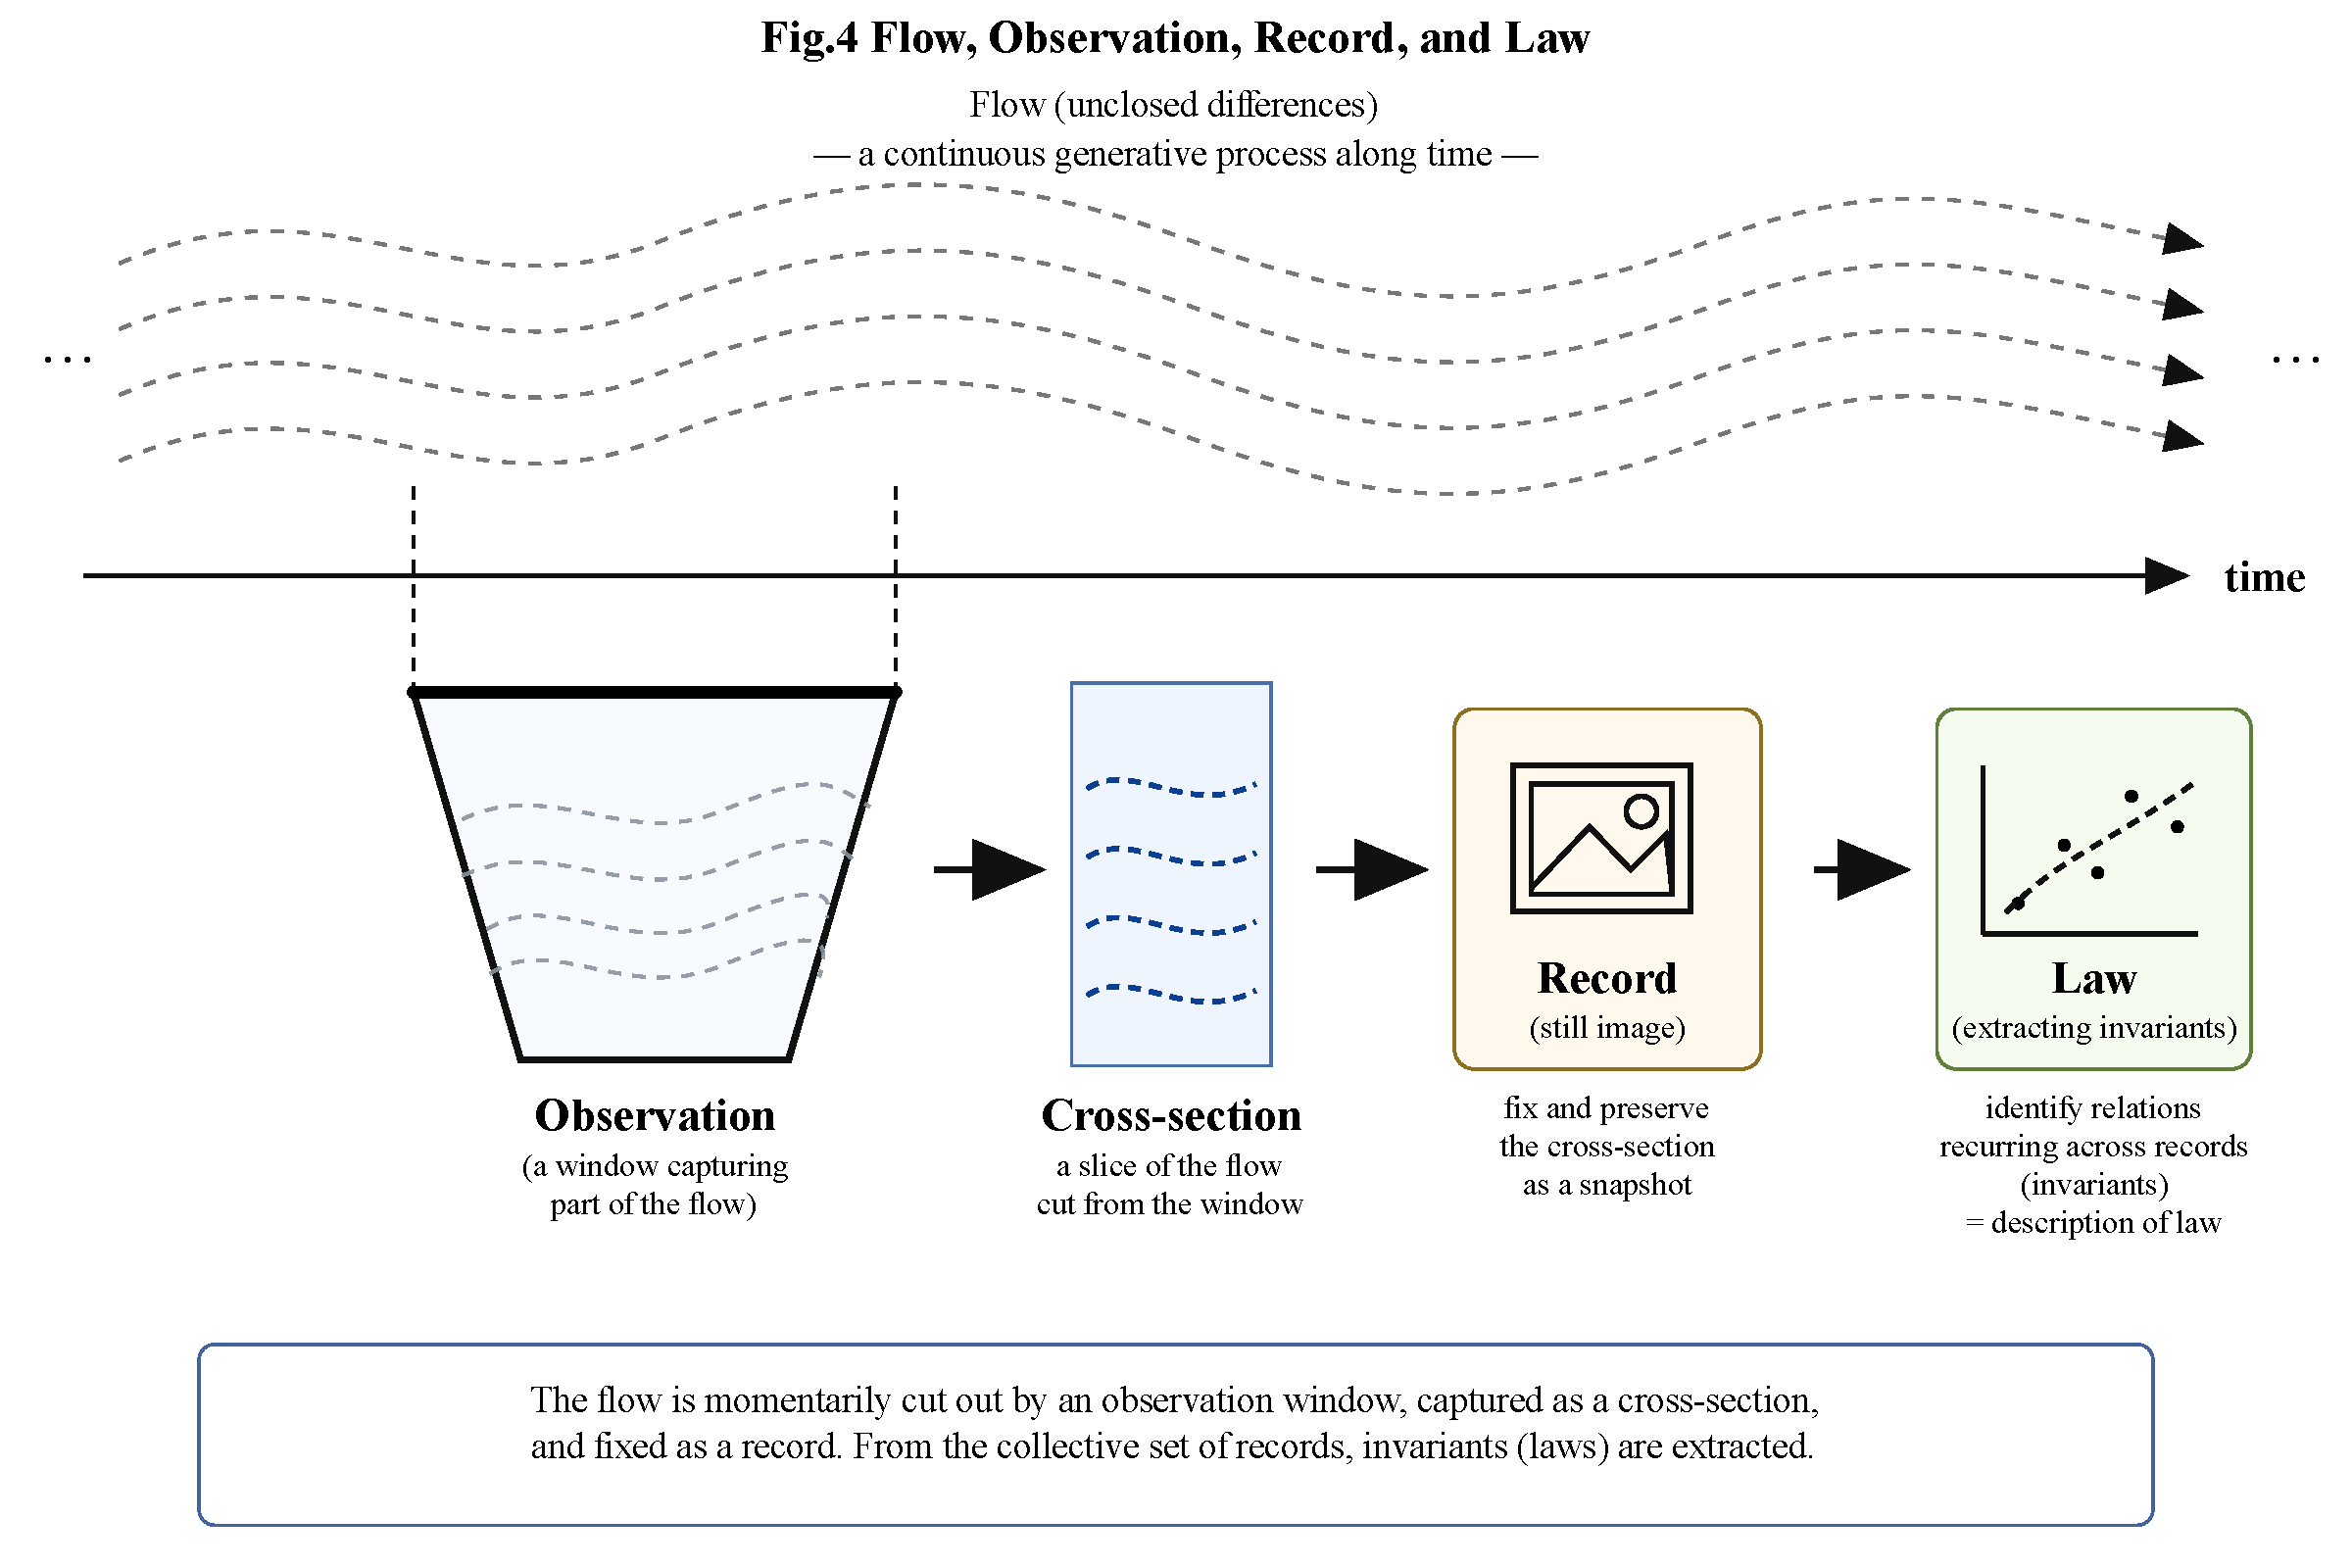
\includegraphics[width=0.88\textwidth]{figures/fig4_observationen_en.pdf}
  \caption{Flow, Observation, Record, and Law.
    The flow is locally cut out by an observation window, captured as a cross-section,
    and fixed as a record.
    From the collective set of records, invariants (laws) are extracted.}
  \label{fig:obs_record_law}
\end{figure}

As a consequence, what is observed appears static.
This apparent stillness is not an intrinsic property of the world itself, but a result of the
observational process.
Even when represented as continuous media such as video or signal streams, observation consists of
a sequence of stabilized cross-sections, rather than direct access to the generative frontier
(see Fig.~\ref{fig:obs_record_law}).

This structure extends naturally to recording.
Recording is not the storage of information as such, but the transformation of differences into
high-closure configurations that can later be reactivated.
Written text, visual imagery, sound, and digital data do not constitute information in themselves;
rather, they function as interference devices that enable the re-emergence of informational
relations.

This perspective also clarifies the status of physical laws.
Laws do not generate the behavior of the world; instead, they are extracted from sequences of
high-closure observational states as stable relations.
That is,
\begin{quote}
  \itshape
  physical laws can be understood as invariants extracted from sequences of high-closure
  cross-sections.
\end{quote}

The apparent stability of the world does not imply simplicity or static structure.
On the contrary, it reflects the existence of a regime in which a large number of invariants
persist across the observational projection of an underlying high-density, high-frequency
dynamical process.
Physical laws are thus traces of dynamical stability, rather than generative principles.

This framework suggests that observable systems should exhibit invariant
structures corresponding to high-closure cross-sections, providing a potential
direction for empirical investigation.

Importantly, this reconfiguration does not invalidate existing physical descriptions.
Atomistic models and law-based formulations remain highly accurate within the domains in which they
operate.
However, they correspond to descriptions in high-closure regimes and do not directly capture the
generative dynamics from which these stable structures emerge.

In the present framework, the starting point is instead placed at a more minimal level:
\begin{quote}
  \itshape
  difference exists.
\end{quote}
From this minimal asymmetry, gradients arise, flows are generated, structures are formed, and
eventually stable invariants appear as observable laws.
In this sense, atoms and laws are not the fundamental drivers of the world, but emergent structures
within an ongoing generative process.

Finally, this perspective offers a natural reinterpretation of classical philosophical problems,
such as Hume's analysis of causation and various thought experiments (e.g., the five-minute
hypothesis or simulation scenarios).
Since observation operates on stabilized configurations, the generative history and origin of a
system are not directly accessible.
These problems thus reflect not a failure of knowledge, but a structural property of observation
itself: it selects high-closure slices of an inherently unclosed process.

Accordingly, the present work does not claim to solve the measurement problem, but rather to
provide an additional structural axis along which it may be reconsidered.
In this context, observation can be understood as an operation that shifts a system toward higher
closure, thereby restricting access to the generative domain that lies toward lower and
intermediate~$C$ (see Eq.~(6) and \S\ref{sec:fundamental_dynamics}).


% ============================================================
%  §7  Conclusion
% ============================================================

\section{Conclusion}
\label{sec:conclusion}

This paper has proposed Information Field Geometry Theory (IFGT) and redefined information as the
structure of a quasi-closure that persists as a trace of difference.
Under this framing, information is understood not as a description of states or an independent
substance, but as a geometric structure that constrains the paths and distributions of difference
chains.

IFGT is positioned as an upper-layer theory built upon the generative structure described by
Vortical Enclosure Dynamics (VED), and it clarifies the correspondence between physical persistence
through closure and informational structure through quasi-closure.
The two are not opposing theories but complementary frameworks describing the same generative
structure from different aspects.
In particular, by formulating the relation between information density~$I$ and closure degree~$C$
as $I = f(1-C)$, the division of roles between the two theories is made explicit at the level of
variables.

The theory introduces the information density~$I$, the information flow~$J$, the information
potential~$\Phi$, the informational time~$\tau$, and the generation term~$\sigma$ to describe
motion within a quasi-closure.
In Section~5, $\sigma$ is expanded into three contributions---driving, dissipation, and
barrier---and a single evolution equation for the closure-degree field~$C(x,\tau)$ is obtained as
the unified VED$\times$IFGT equation~(11).
This equation is derived from two minimal axioms: \emph{there is difference} and \emph{difference
tends to close}.

Within this framework, information appears not as a static object of description, but as a dynamic
process that participates in structural formation through the persistence of difference and the
constraint of flow.
Physical structure and informational structure are not separated entities; they are understood as
being generated cyclically through mutual influence.

The scope of the IFGT concept of information relative to existing frameworks is summarized in
Fig.~\ref{fig:coverage_map}: IFGT addresses the full continuum of closure degree~$C$, integrating
the domains covered by Shannon information, affordance, common-sense information, and physical
information into a single dynamical description.

\begin{figure}[h]
  \centering
  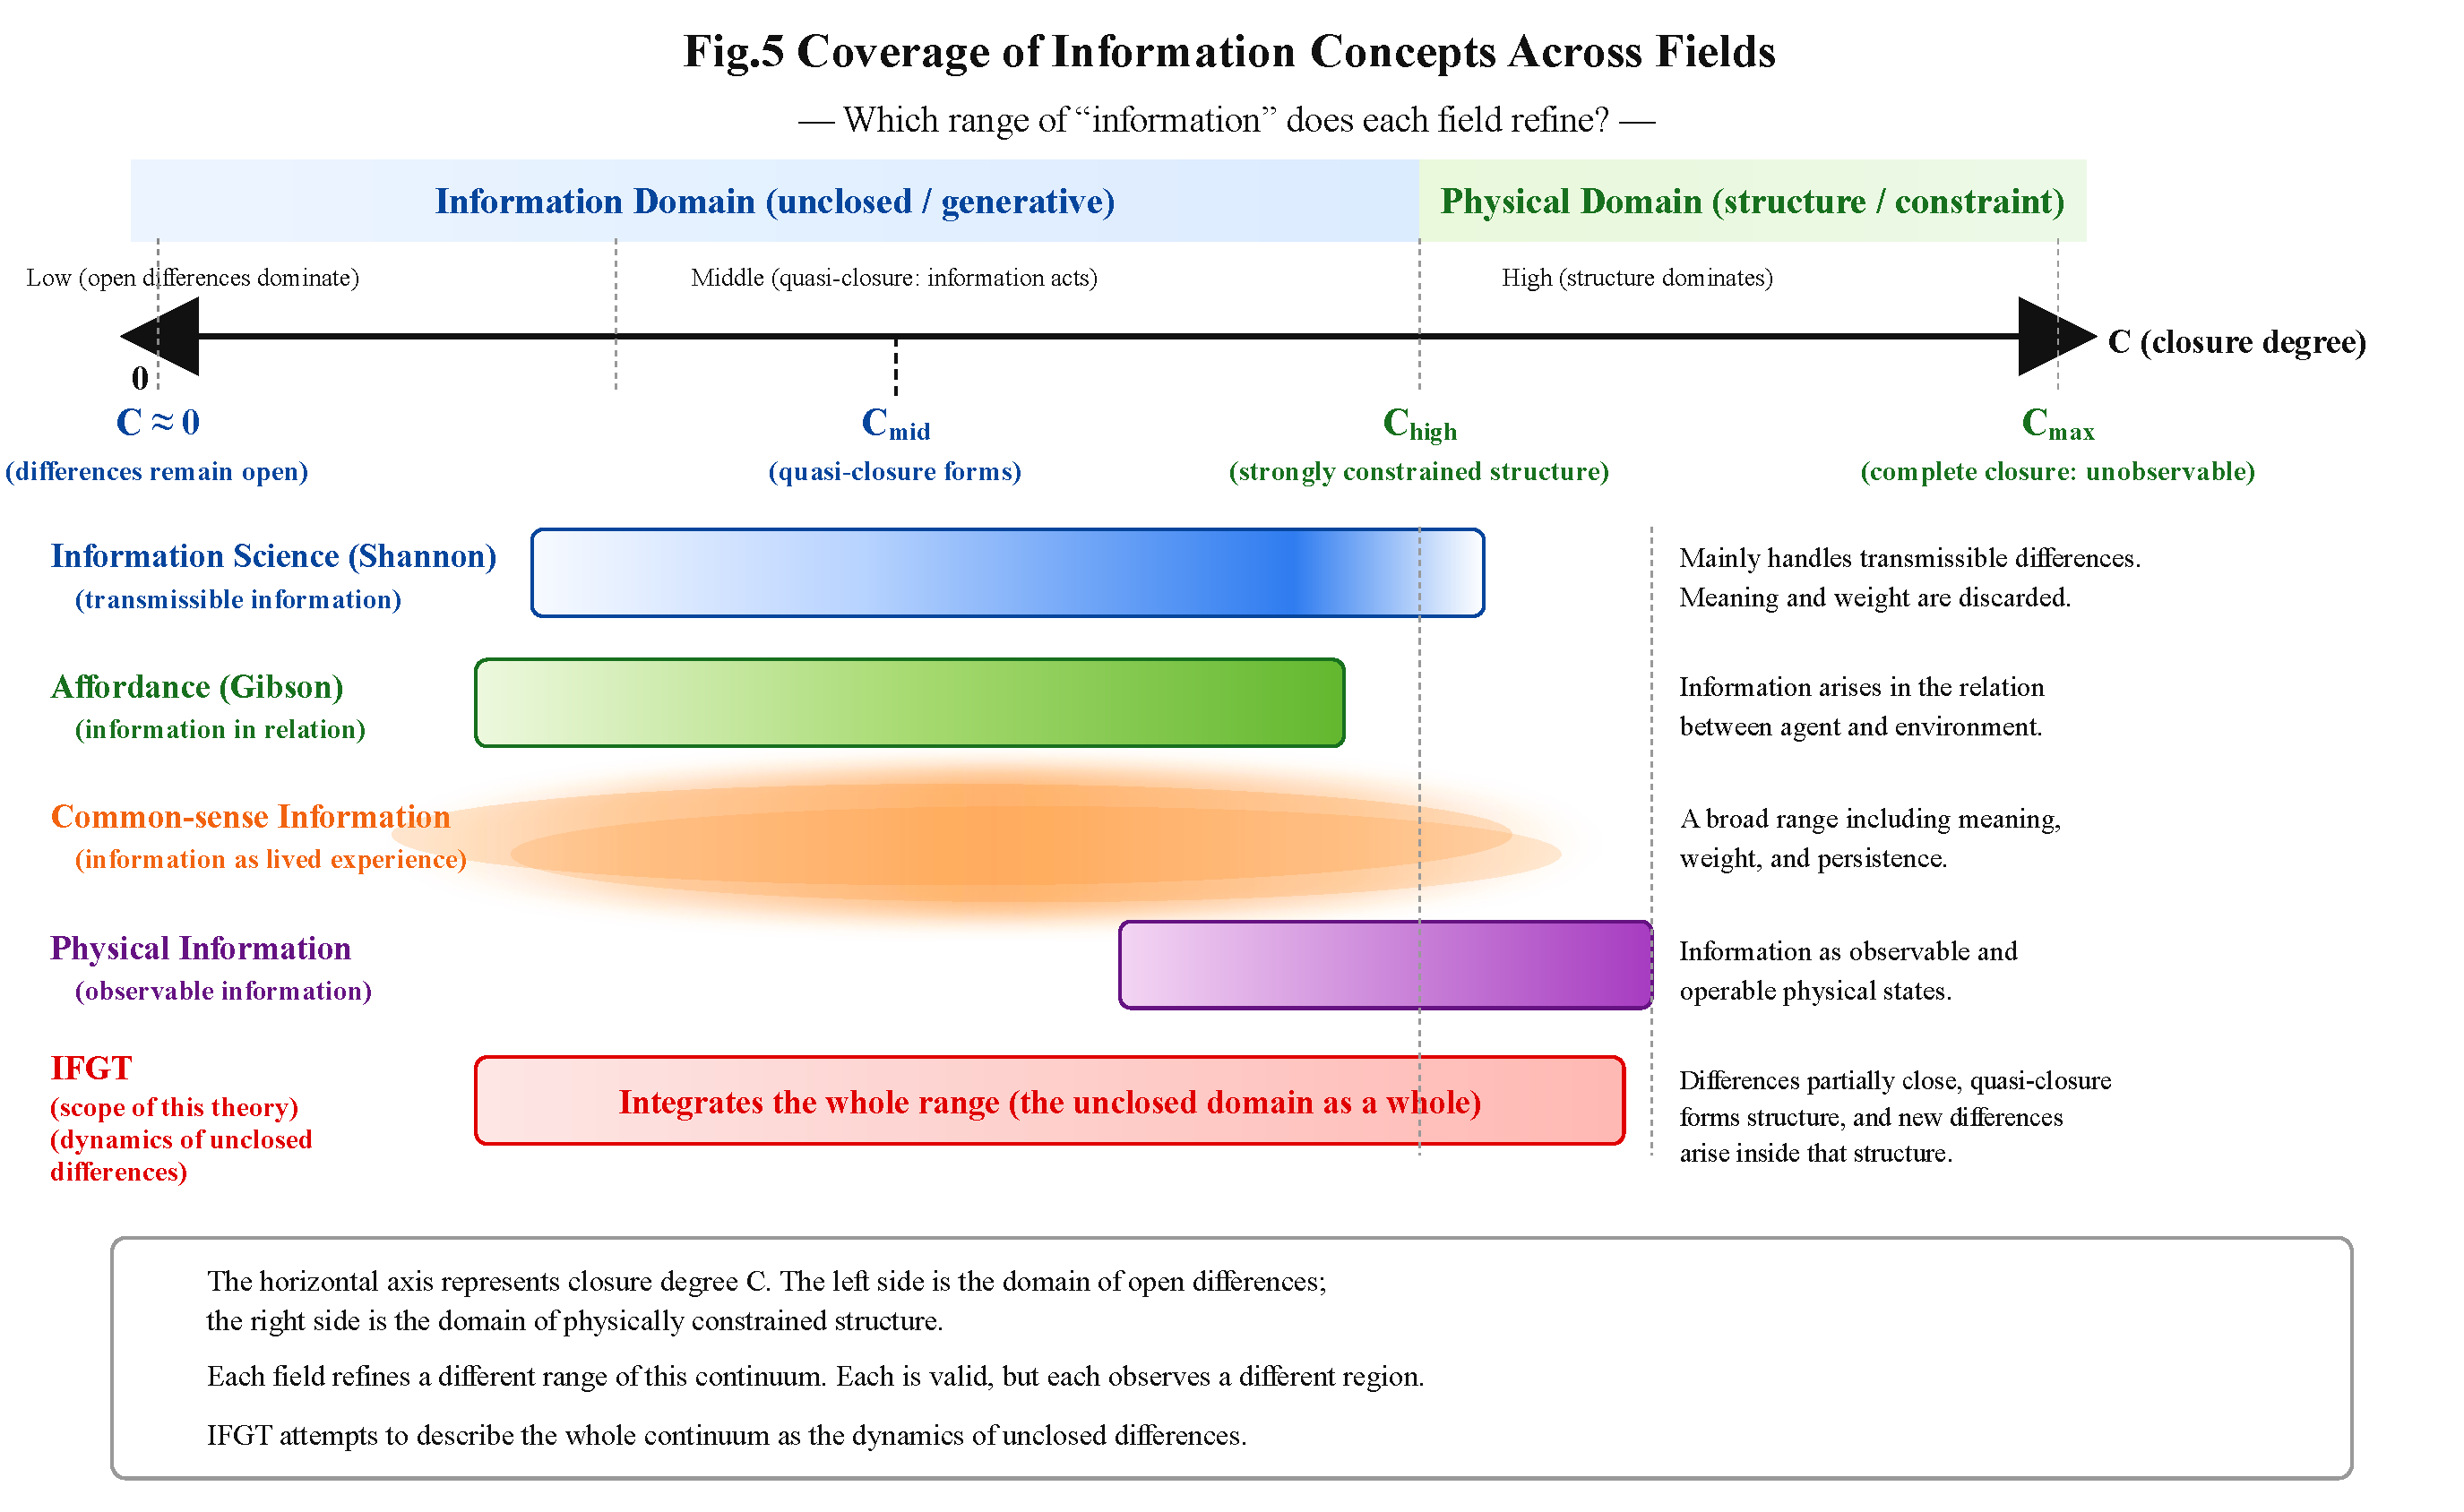
\includegraphics[width=0.92\textwidth]{figures/fig5_information_coverage_map_recreated_en.pdf}
  \caption{Coverage of information concepts across fields.
    The horizontal axis represents closure degree~$C$.
    Each field refines a different range of this continuum.
    IFGT attempts to describe the whole continuum as the dynamics of unclosed differences.}
  \label{fig:coverage_map}
\end{figure}

This paper has not addressed the concrete implementations in biological or computational systems,
but the structure described by IFGT is suggested to appear prominently in such systems.
The theory aims at a general description of structure that does not depend on any particular domain.

The scope of the theory is, at present, limited to the minimal description of informational
structure and the introduction of the unified equation.
Further developments may include the correspondence with concrete structures in domains such as
life, consciousness, language, and intelligence, as well as detailed analysis of the unified
equation~(11) (classification of stable solutions, existence conditions for limit-cycle solutions,
renormalization structure, and so on), but these lie beyond the direct scope of this paper.

In sum, IFGT provides a minimal theory for describing, as geometry, the motion of quasi-closure
that persists in the process by which structure is generated from difference.
This paper presents its foundational framework; detailed developments and applications remain as
future work.


\bibliographystyle{plain}
\bibliography{refs}

\end{document}
